\documentclass{article}

\usepackage[utf8]{inputenc}
\usepackage[letterpaper, total={6in, 9in}]{geometry}
\usepackage{amsmath}
\usepackage{natbib}
\usepackage{wrapfig}
\usepackage{graphicx}
\usepackage{amssymb}
\usepackage{tikz}

\title{Geometry 4 - Analytic Geomtry}
\author{TSS Math Club}
\date{Nov 2022}

\begin{document}

\maketitle

\section{Preliminary}

% \subsection{Field}

% \subsubsection{Definition}

% \begin{itemize}
%     \item Associativity of addition and multiplication:
%     \item Commutativity of addition and multiplication:
%     \item Additive and multiplicative identity:
%     \item Additive inverses:
%     \item Multiplicative inverses:
%     \item Distributivity of multiplication over addition:
% \end{itemize}

\subsection{Real Line}

\subsubsection{Definition}

A number line is a picture of a graduated straight line that serves as visual representation of the real numbers. Every point of a number line is assumed to correspond to a real number, and every real number to a point.



\tikzset{every picture/.style={line width=0.75pt}} %set default line width to 0.75pt        

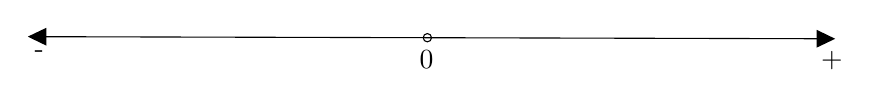
\begin{tikzpicture}[x=0.75pt,y=0.75pt,yscale=-1,xscale=1]
%uncomment if require: \path (0,411); %set diagram left start at 0, and has height of 411

%Straight Lines [id:da37370818120152194] 
\draw    (103,122.01) -- (486.01,123.02) ;
\draw [shift={(489.01,123.03)}, rotate = 180.15] [fill={rgb, 255:red, 0; green, 0; blue, 0 }  ][line width=0.08]  [draw opacity=0] (8.93,-4.29) -- (0,0) -- (8.93,4.29) -- cycle    ;
\draw [shift={(100,122)}, rotate = 0.15] [fill={rgb, 255:red, 0; green, 0; blue, 0 }  ][line width=0.08]  [draw opacity=0] (8.93,-4.29) -- (0,0) -- (8.93,4.29) -- cycle    ;
%Shape: Circle [id:dp6550024446713398] 
\draw   (290.52,122.51) .. controls (290.52,121.41) and (291.41,120.52) .. (292.51,120.52) .. controls (293.62,120.52) and (294.51,121.41) .. (294.51,122.51) .. controls (294.51,123.61) and (293.62,124.51) .. (292.51,124.51) .. controls (291.41,124.51) and (290.52,123.61) .. (290.52,122.51) -- cycle ;

% Text Node
\draw (287.51,127.51) node [anchor=north west][inner sep=0.75pt]   [align=left] {0};
% Text Node
\draw (481,128) node [anchor=north west][inner sep=0.75pt]   [align=left] {+};
% Text Node
\draw (102,125) node [anchor=north west][inner sep=0.75pt]   [align=left] {\mbox{-}};


\end{tikzpicture}


\subsection{Ordered Pair}

\subsubsection{Definition}

Informal:
\begin{quote}
For any two objects a and b, the ordered pair (a, b) is a notation specifying the two objects a and b, in that order.
\end{quote}
Formal:
\begin{quote}
(a,b)=\{\{a\},\{a,b\}\}
\end{quote}

\subsubsection{Property}

$$(a,b)=(c,d) \iff a=c \land b=d$$

\subsection{Cartesian Product}

\subsubsection{Definition}

The Cartesian product of two sets $A$ and $B$, denoted $A \times B$, is the set of all ordered pairs $(a, b)$ where $a$ is in $A$ and $b$ is in $B$.

$$A \times B = \{(a,b) \mid a \in A, b \in B \}$$


\section{Cartesian Plane}

\subsection{Definition}


\pagebreak

\subsection{Visual Representation}



\tikzset{every picture/.style={line width=0.75pt}} %set default line width to 0.75pt        

\begin{tikzpicture}[x=0.75pt,y=0.75pt,yscale=-.7,xscale=.7]
%uncomment if require: \path (0,300); %set diagram left start at 0, and has height of 300

%Straight Lines [id:da5485385098063555] 
\draw    (256.01,257.03) -- (256.01,26.03) ;
\draw [shift={(256.01,24.03)}, rotate = 90] [color={rgb, 255:red, 0; green, 0; blue, 0 }  ][line width=0.75]    (10.93,-3.29) .. controls (6.95,-1.4) and (3.31,-0.3) .. (0,0) .. controls (3.31,0.3) and (6.95,1.4) .. (10.93,3.29)   ;
%Straight Lines [id:da9244581279454482] 
\draw    (95.01,161.03) -- (433.01,160.03) ;
\draw [shift={(435.01,160.03)}, rotate = 179.83] [color={rgb, 255:red, 0; green, 0; blue, 0 }  ][line width=0.75]    (10.93,-3.29) .. controls (6.95,-1.4) and (3.31,-0.3) .. (0,0) .. controls (3.31,0.3) and (6.95,1.4) .. (10.93,3.29)   ;




\end{tikzpicture}


\subsection{Point}
\subsubsection{Definition}
\vspace{20px}

\subsubsection{Plot points}



\tikzset{every picture/.style={line width=0.75pt}} %set default line width to 0.75pt        

\begin{tikzpicture}[x=0.75pt,y=0.75pt,yscale=-.7,xscale=.7]
%uncomment if require: \path (0,300); %set diagram left start at 0, and has height of 300

%Straight Lines [id:da5485385098063555] 
\draw    (137.67,209.03) -- (137.67,45.03) ;
\draw [shift={(137.67,43.03)}, rotate = 90] [color={rgb, 255:red, 0; green, 0; blue, 0 }  ][line width=0.75]    (10.93,-3.29) .. controls (6.95,-1.4) and (3.31,-0.3) .. (0,0) .. controls (3.31,0.3) and (6.95,1.4) .. (10.93,3.29)   ;
%Straight Lines [id:da9244581279454482] 
\draw    (42.01,140.63) -- (242.01,139.93) ;
\draw [shift={(244.01,139.92)}, rotate = 179.8] [color={rgb, 255:red, 0; green, 0; blue, 0 }  ][line width=0.75]    (10.93,-3.29) .. controls (6.95,-1.4) and (3.31,-0.3) .. (0,0) .. controls (3.31,0.3) and (6.95,1.4) .. (10.93,3.29)   ;
%Straight Lines [id:da2006977343179377] 
\draw    (439.67,210.03) -- (439.67,46.03) ;
\draw [shift={(439.67,44.03)}, rotate = 90] [color={rgb, 255:red, 0; green, 0; blue, 0 }  ][line width=0.75]    (10.93,-3.29) .. controls (6.95,-1.4) and (3.31,-0.3) .. (0,0) .. controls (3.31,0.3) and (6.95,1.4) .. (10.93,3.29)   ;
%Straight Lines [id:da9562220195154991] 
\draw    (344.01,141.63) -- (544.01,140.93) ;
\draw [shift={(546.01,140.92)}, rotate = 179.8] [color={rgb, 255:red, 0; green, 0; blue, 0 }  ][line width=0.75]    (10.93,-3.29) .. controls (6.95,-1.4) and (3.31,-0.3) .. (0,0) .. controls (3.31,0.3) and (6.95,1.4) .. (10.93,3.29)   ;

% Text Node
\draw (121,223) node [anchor=north west][inner sep=0.75pt]   [align=left] {(3,5)};
% Text Node
\draw (420.67,221.03) node [anchor=north west][inner sep=0.75pt]   [align=left] {(-6,2)};


\end{tikzpicture}


\subsection{Metric on the Plane}
\subsubsection{Distance formula}



\tikzset{every picture/.style={line width=0.75pt}} %set default line width to 0.75pt        

\begin{tikzpicture}[x=0.75pt,y=0.75pt,yscale=-.7,xscale=.7]
%uncomment if require: \path (0,300); %set diagram left start at 0, and has height of 300

%Straight Lines [id:da5485385098063555] 
\draw    (181.01,267.03) -- (181.01,36.03) ;
\draw [shift={(181.01,34.03)}, rotate = 90] [color={rgb, 255:red, 0; green, 0; blue, 0 }  ][line width=0.75]    (10.93,-3.29) .. controls (6.95,-1.4) and (3.31,-0.3) .. (0,0) .. controls (3.31,0.3) and (6.95,1.4) .. (10.93,3.29)   ;
%Straight Lines [id:da9244581279454482] 
\draw    (115.01,225.03) -- (453.01,224.03) ;
\draw [shift={(455.01,224.03)}, rotate = 179.83] [color={rgb, 255:red, 0; green, 0; blue, 0 }  ][line width=0.75]    (10.93,-3.29) .. controls (6.95,-1.4) and (3.31,-0.3) .. (0,0) .. controls (3.31,0.3) and (6.95,1.4) .. (10.93,3.29)   ;
%Straight Lines [id:da9012580532288677] 
\draw    (328.01,96.03) -- (228.01,174.03) ;

% Text Node
\draw (230.01,177.03) node [anchor=north west][inner sep=0.75pt]   [align=left] {(x1,y1)};
% Text Node
\draw (330.01,99.03) node [anchor=north west][inner sep=0.75pt]   [align=left] {(x2,y2)};


\end{tikzpicture}

\vspace{30px}

\subsubsection{Example}

Find the distance between (1,3) and (6,7).


\pagebreak

\subsection{Line}
\subsubsection{General Formula}
\vspace{20px}
\subsubsection{Examples}

\tikzset{every picture/.style={line width=0.75pt}} %set default line width to 0.75pt        

\begin{tikzpicture}[x=0.75pt,y=0.75pt,yscale=-1,xscale=1]
%uncomment if require: \path (0,300); %set diagram left start at 0, and has height of 300

%Straight Lines [id:da5485385098063555] 
\draw    (156.93,207.03) -- (156.93,49.03) ;
\draw [shift={(156.93,47.03)}, rotate = 90] [color={rgb, 255:red, 0; green, 0; blue, 0 }  ][line width=0.75]    (10.93,-3.29) .. controls (6.95,-1.4) and (3.31,-0.3) .. (0,0) .. controls (3.31,0.3) and (6.95,1.4) .. (10.93,3.29)   ;
%Straight Lines [id:da9244581279454482] 
\draw    (57.01,141.1) -- (266.01,140.42) ;
\draw [shift={(268.01,140.42)}, rotate = 179.81] [color={rgb, 255:red, 0; green, 0; blue, 0 }  ][line width=0.75]    (10.93,-3.29) .. controls (6.95,-1.4) and (3.31,-0.3) .. (0,0) .. controls (3.31,0.3) and (6.95,1.4) .. (10.93,3.29)   ;
%Straight Lines [id:da40962903604479894] 
\draw    (401.93,207.03) -- (401.93,49.03) ;
\draw [shift={(401.93,47.03)}, rotate = 90] [color={rgb, 255:red, 0; green, 0; blue, 0 }  ][line width=0.75]    (10.93,-3.29) .. controls (6.95,-1.4) and (3.31,-0.3) .. (0,0) .. controls (3.31,0.3) and (6.95,1.4) .. (10.93,3.29)   ;
%Straight Lines [id:da02167311792978177] 
\draw    (302.01,141.1) -- (511.01,140.42) ;
\draw [shift={(513.01,140.42)}, rotate = 179.81] [color={rgb, 255:red, 0; green, 0; blue, 0 }  ][line width=0.75]    (10.93,-3.29) .. controls (6.95,-1.4) and (3.31,-0.3) .. (0,0) .. controls (3.31,0.3) and (6.95,1.4) .. (10.93,3.29)   ;
%Straight Lines [id:da7739113600191492] 
\draw    (294.54,181.41) -- (484.49,59.65) ;
\draw [shift={(487.01,58.03)}, rotate = 147.34] [fill={rgb, 255:red, 0; green, 0; blue, 0 }  ][line width=0.08]  [draw opacity=0] (10.72,-5.15) -- (0,0) -- (10.72,5.15) -- (7.12,0) -- cycle    ;
\draw [shift={(292.01,183.03)}, rotate = 327.34] [fill={rgb, 255:red, 0; green, 0; blue, 0 }  ][line width=0.08]  [draw opacity=0] (10.72,-5.15) -- (0,0) -- (10.72,5.15) -- (7.12,0) -- cycle    ;

% Text Node
\draw (114,215) node [anchor=north west][inner sep=0.75pt]   [align=left] {3x+4y+12=0};
% Text Node
\draw (402,114) node [anchor=north west][inner sep=0.75pt]   [align=left] {(0,2)};
% Text Node
\draw (354,143) node [anchor=north west][inner sep=0.75pt]   [align=left] {(-4,0)};


\end{tikzpicture}


\subsection{Circle}

\subsubsection{General Formula}
\vspace{20px}

\subsubsection{Examples}


\tikzset{every picture/.style={line width=0.75pt}} %set default line width to 0.75pt        

\begin{tikzpicture}[x=0.75pt,y=0.75pt,yscale=-1,xscale=1]
%uncomment if require: \path (0,300); %set diagram left start at 0, and has height of 300

%Straight Lines [id:da5485385098063555] 
\draw    (156.93,207.03) -- (156.93,49.03) ;
\draw [shift={(156.93,47.03)}, rotate = 90] [color={rgb, 255:red, 0; green, 0; blue, 0 }  ][line width=0.75]    (10.93,-3.29) .. controls (6.95,-1.4) and (3.31,-0.3) .. (0,0) .. controls (3.31,0.3) and (6.95,1.4) .. (10.93,3.29)   ;
%Straight Lines [id:da9244581279454482] 
\draw    (57.01,141.1) -- (266.01,140.42) ;
\draw [shift={(268.01,140.42)}, rotate = 179.81] [color={rgb, 255:red, 0; green, 0; blue, 0 }  ][line width=0.75]    (10.93,-3.29) .. controls (6.95,-1.4) and (3.31,-0.3) .. (0,0) .. controls (3.31,0.3) and (6.95,1.4) .. (10.93,3.29)   ;
%Straight Lines [id:da40962903604479894] 
\draw    (401.93,207.03) -- (401.93,49.03) ;
\draw [shift={(401.93,47.03)}, rotate = 90] [color={rgb, 255:red, 0; green, 0; blue, 0 }  ][line width=0.75]    (10.93,-3.29) .. controls (6.95,-1.4) and (3.31,-0.3) .. (0,0) .. controls (3.31,0.3) and (6.95,1.4) .. (10.93,3.29)   ;
%Straight Lines [id:da02167311792978177] 
\draw    (302.01,141.1) -- (511.01,140.42) ;
\draw [shift={(513.01,140.42)}, rotate = 179.81] [color={rgb, 255:red, 0; green, 0; blue, 0 }  ][line width=0.75]    (10.93,-3.29) .. controls (6.95,-1.4) and (3.31,-0.3) .. (0,0) .. controls (3.31,0.3) and (6.95,1.4) .. (10.93,3.29)   ;
%Shape: Circle [id:dp6957597863561313] 
\draw   (423.97,94.01) .. controls (423.97,76.89) and (437.86,63) .. (454.99,63) .. controls (472.11,63) and (486,76.89) .. (486,94.01) .. controls (486,111.14) and (472.11,125.03) .. (454.99,125.03) .. controls (437.86,125.03) and (423.97,111.14) .. (423.97,94.01) -- cycle ;
%Straight Lines [id:da35029674067957206] 
\draw    (486.01,117.03) -- (456.59,95.2) ;
\draw [shift={(454.99,94.01)}, rotate = 36.56] [color={rgb, 255:red, 0; green, 0; blue, 0 }  ][line width=0.75]    (10.93,-3.29) .. controls (6.95,-1.4) and (3.31,-0.3) .. (0,0) .. controls (3.31,0.3) and (6.95,1.4) .. (10.93,3.29)   ;

% Text Node
\draw (86,214) node [anchor=north west][inner sep=0.75pt]   [align=left] {x\textasciicircum 2+2x+y\textasciicircum 2+4x+2=0};
% Text Node
\draw (486.99,108.01) node [anchor=north west][inner sep=0.75pt]   [align=left] {(3,4)};
% Text Node
\draw (485,69) node [anchor=north west][inner sep=0.75pt]   [align=left] {r=1};


\end{tikzpicture}

\subsection{Point to Line DIstance Formula}

The distance between the line $ax+by+c = 0$ and point $(x_1,y_1)$ is\[\dfrac{|ax_1+by_1+c|}{\sqrt{a^2+b^2}}\]

\pagebreak


\subsection{Intersection}
\subsubsection{How to find intersection between two curve?}
\vspace{20px}
\subsubsection{Example}


\tikzset{every picture/.style={line width=0.75pt}} %set default line width to 0.75pt        

\begin{tikzpicture}[x=0.75pt,y=0.75pt,yscale=-.8,xscale=.8]
%uncomment if require: \path (0,300); %set diagram left start at 0, and has height of 300

%Straight Lines [id:da40962903604479894] 
\draw    (259.01,280.03) -- (259.01,38.03) ;
\draw [shift={(259.01,36.03)}, rotate = 90] [color={rgb, 255:red, 0; green, 0; blue, 0 }  ][line width=0.75]    (10.93,-3.29) .. controls (6.95,-1.4) and (3.31,-0.3) .. (0,0) .. controls (3.31,0.3) and (6.95,1.4) .. (10.93,3.29)   ;
%Straight Lines [id:da02167311792978177] 
\draw    (98.01,179.49) -- (436.01,178.45) ;
\draw [shift={(438.01,178.45)}, rotate = 179.82] [color={rgb, 255:red, 0; green, 0; blue, 0 }  ][line width=0.75]    (10.93,-3.29) .. controls (6.95,-1.4) and (3.31,-0.3) .. (0,0) .. controls (3.31,0.3) and (6.95,1.4) .. (10.93,3.29)   ;
%Shape: Ellipse [id:dp6957597863561313] 
\draw   (309.54,102.68) .. controls (309.54,76.56) and (331.91,55.39) .. (359.51,55.39) .. controls (387.11,55.39) and (409.48,76.56) .. (409.48,102.68) .. controls (409.48,128.8) and (387.11,149.98) .. (359.51,149.98) .. controls (331.91,149.98) and (309.54,128.8) .. (309.54,102.68) -- cycle ;
%Straight Lines [id:da9711457273086297] 
\draw    (130.01,235.03) -- (444.01,9.03) ;

% Text Node
\draw (398,133) node [anchor=north west][inner sep=0.75pt]   [align=left] {(x-4)\textasciicircum 2+(y-3)\textasciicircum 2=2};
% Text Node
\draw (402,43) node [anchor=north west][inner sep=0.75pt]   [align=left] {2x-y=4};


\end{tikzpicture}

\vspace{100px}

\subsubsection{Find the Radical Axis of Two Circles}
Definition: \\ \\ \\
Find the radical axis bewteen $x^2+y^2=5$ and $x^2+3x+y^2-7y+3=0$.



\pagebreak

\section{Vector}
\subsection{Definition}
\vspace{20px}
\subsection{Visual Representation}


\tikzset{every picture/.style={line width=0.75pt}} %set default line width to 0.75pt        

\begin{tikzpicture}[x=0.75pt,y=0.75pt,yscale=-.7,xscale=.7]
%uncomment if require: \path (0,300); %set diagram left start at 0, and has height of 300

%Straight Lines [id:da40962903604479894] 
\draw    (259.01,280.03) -- (259.01,38.03) ;
\draw [shift={(259.01,36.03)}, rotate = 90] [color={rgb, 255:red, 0; green, 0; blue, 0 }  ][line width=0.75]    (10.93,-3.29) .. controls (6.95,-1.4) and (3.31,-0.3) .. (0,0) .. controls (3.31,0.3) and (6.95,1.4) .. (10.93,3.29)   ;
%Straight Lines [id:da02167311792978177] 
\draw    (98.01,179.49) -- (436.01,178.45) ;
\draw [shift={(438.01,178.45)}, rotate = 179.82] [color={rgb, 255:red, 0; green, 0; blue, 0 }  ][line width=0.75]    (10.93,-3.29) .. controls (6.95,-1.4) and (3.31,-0.3) .. (0,0) .. controls (3.31,0.3) and (6.95,1.4) .. (10.93,3.29)   ;
%Straight Lines [id:da7156592326299953] 
\draw    (258.01,179.03) -- (341.27,132.01) ;
\draw [shift={(343.01,131.03)}, rotate = 150.55] [color={rgb, 255:red, 0; green, 0; blue, 0 }  ][line width=0.75]    (10.93,-3.29) .. controls (6.95,-1.4) and (3.31,-0.3) .. (0,0) .. controls (3.31,0.3) and (6.95,1.4) .. (10.93,3.29)   ;


\end{tikzpicture}

\subsection{Addition, Substraction and Scalar Multiplication of Vectors}
\subsubsection{Addition of Vectors}
Algebra:\\ \\
Geometry:


\tikzset{every picture/.style={line width=0.75pt}} %set default line width to 0.75pt        

\begin{tikzpicture}[x=0.75pt,y=0.75pt,yscale=-.6,xscale=.6]
%uncomment if require: \path (0,300); %set diagram left start at 0, and has height of 300

%Straight Lines [id:da40962903604479894] 
\draw    (259.01,280.03) -- (259.01,38.03) ;
\draw [shift={(259.01,36.03)}, rotate = 90] [color={rgb, 255:red, 0; green, 0; blue, 0 }  ][line width=0.75]    (10.93,-3.29) .. controls (6.95,-1.4) and (3.31,-0.3) .. (0,0) .. controls (3.31,0.3) and (6.95,1.4) .. (10.93,3.29)   ;
%Straight Lines [id:da02167311792978177] 
\draw    (98.01,179.49) -- (436.01,178.45) ;
\draw [shift={(438.01,178.45)}, rotate = 179.82] [color={rgb, 255:red, 0; green, 0; blue, 0 }  ][line width=0.75]    (10.93,-3.29) .. controls (6.95,-1.4) and (3.31,-0.3) .. (0,0) .. controls (3.31,0.3) and (6.95,1.4) .. (10.93,3.29)   ;
%Straight Lines [id:da7156592326299953] 
\draw    (258.01,179.03) -- (300.89,115.68) ;
\draw [shift={(302.01,114.03)}, rotate = 124.09] [color={rgb, 255:red, 0; green, 0; blue, 0 }  ][line width=0.75]    (10.93,-3.29) .. controls (6.95,-1.4) and (3.31,-0.3) .. (0,0) .. controls (3.31,0.3) and (6.95,1.4) .. (10.93,3.29)   ;
%Straight Lines [id:da4792480491525051] 
\draw    (258.01,179.03) -- (339.41,239.83) ;
\draw [shift={(341.01,241.03)}, rotate = 216.76] [color={rgb, 255:red, 0; green, 0; blue, 0 }  ][line width=0.75]    (10.93,-3.29) .. controls (6.95,-1.4) and (3.31,-0.3) .. (0,0) .. controls (3.31,0.3) and (6.95,1.4) .. (10.93,3.29)   ;

% Text Node
\draw (282.01,149.53) node [anchor=north west][inner sep=0.75pt]   [align=left] {u};
% Text Node
\draw (301.51,213.03) node [anchor=north west][inner sep=0.75pt]   [align=left] {v};


\end{tikzpicture}

\subsubsection{Substraction of Vectors}
Algebra:\\ \\
Geometry:


\tikzset{every picture/.style={line width=0.75pt}} %set default line width to 0.75pt        

\begin{tikzpicture}[x=0.75pt,y=0.75pt,yscale=-.6,xscale=.6]
%uncomment if require: \path (0,300); %set diagram left start at 0, and has height of 300

%Straight Lines [id:da40962903604479894] 
\draw    (259.01,280.03) -- (259.01,38.03) ;
\draw [shift={(259.01,36.03)}, rotate = 90] [color={rgb, 255:red, 0; green, 0; blue, 0 }  ][line width=0.75]    (10.93,-3.29) .. controls (6.95,-1.4) and (3.31,-0.3) .. (0,0) .. controls (3.31,0.3) and (6.95,1.4) .. (10.93,3.29)   ;
%Straight Lines [id:da02167311792978177] 
\draw    (98.01,179.49) -- (436.01,178.45) ;
\draw [shift={(438.01,178.45)}, rotate = 179.82] [color={rgb, 255:red, 0; green, 0; blue, 0 }  ][line width=0.75]    (10.93,-3.29) .. controls (6.95,-1.4) and (3.31,-0.3) .. (0,0) .. controls (3.31,0.3) and (6.95,1.4) .. (10.93,3.29)   ;
%Straight Lines [id:da7156592326299953] 
\draw    (258.01,179.03) -- (300.89,115.68) ;
\draw [shift={(302.01,114.03)}, rotate = 124.09] [color={rgb, 255:red, 0; green, 0; blue, 0 }  ][line width=0.75]    (10.93,-3.29) .. controls (6.95,-1.4) and (3.31,-0.3) .. (0,0) .. controls (3.31,0.3) and (6.95,1.4) .. (10.93,3.29)   ;
%Straight Lines [id:da4792480491525051] 
\draw    (258.01,179.03) -- (339.41,239.83) ;
\draw [shift={(341.01,241.03)}, rotate = 216.76] [color={rgb, 255:red, 0; green, 0; blue, 0 }  ][line width=0.75]    (10.93,-3.29) .. controls (6.95,-1.4) and (3.31,-0.3) .. (0,0) .. controls (3.31,0.3) and (6.95,1.4) .. (10.93,3.29)   ;

% Text Node
\draw (282.01,149.53) node [anchor=north west][inner sep=0.75pt]   [align=left] {u};
% Text Node
\draw (301.51,213.03) node [anchor=north west][inner sep=0.75pt]   [align=left] {v};


\end{tikzpicture}

\subsubsection{Scalar Multiplication of Vector}

Algebra:\\ \\
Geometry:


\tikzset{every picture/.style={line width=0.75pt}} %set default line width to 0.75pt        

\begin{tikzpicture}[x=0.75pt,y=0.75pt,yscale=-.6,xscale=.6]
%uncomment if require: \path (0,300); %set diagram left start at 0, and has height of 300

%Straight Lines [id:da40962903604479894] 
\draw    (259.01,280.03) -- (259.01,38.03) ;
\draw [shift={(259.01,36.03)}, rotate = 90] [color={rgb, 255:red, 0; green, 0; blue, 0 }  ][line width=0.75]    (10.93,-3.29) .. controls (6.95,-1.4) and (3.31,-0.3) .. (0,0) .. controls (3.31,0.3) and (6.95,1.4) .. (10.93,3.29)   ;
%Straight Lines [id:da02167311792978177] 
\draw    (98.01,179.49) -- (436.01,178.45) ;
\draw [shift={(438.01,178.45)}, rotate = 179.82] [color={rgb, 255:red, 0; green, 0; blue, 0 }  ][line width=0.75]    (10.93,-3.29) .. controls (6.95,-1.4) and (3.31,-0.3) .. (0,0) .. controls (3.31,0.3) and (6.95,1.4) .. (10.93,3.29)   ;
%Straight Lines [id:da7156592326299953] 
\draw    (258.01,179.03) -- (300.89,115.68) ;
\draw [shift={(302.01,114.03)}, rotate = 124.09] [color={rgb, 255:red, 0; green, 0; blue, 0 }  ][line width=0.75]    (10.93,-3.29) .. controls (6.95,-1.4) and (3.31,-0.3) .. (0,0) .. controls (3.31,0.3) and (6.95,1.4) .. (10.93,3.29)   ;

% Text Node
\draw (282.01,149.53) node [anchor=north west][inner sep=0.75pt]   [align=left] {u};


\end{tikzpicture}


\subsection{Dot Product}

\subsubsection{Definition: Dot Product on 2D}
If $x =(x_1,x_2)$ and $y=(y_1,y_2)$, then
$$x \cdot y = x_1y_1+x_2y_2$$

\subsubsection{Property: Dot Product}
\begin{itemize}
    \item positivity:
    \item definiteness:
    \item additivity:
    \item homogeneity:
    \item symmetry:
\end{itemize}
\subsubsection{Dot Product and Metric}
\vspace{30px}
\subsubsection{Penpendicularity}
\vspace{30px}
\subsubsection{Dot Product and Cosine Law}
\vspace{100px}
\subsubsection{Dot Product as Projection}
\pagebreak
\subsubsection{Problem (1975 USAMO Q2)}
Let $A,B,C,D$ denote four points in space and $AB$ the distance between $A$ and $B$, and so on. Show that\[AC^2+BD^2+AD^2+BC^2\ge AB^2+CD^2.\]

\pagebreak

\subsection{Determinant}
\subsubsection{Definition}
\vspace*{20px}
\subsubsection{Formula}

$
\begin{vmatrix}
    a & b\\
    c & d
\end{vmatrix}
=
$

\subsubsection{3D Determinant and Area of a Triangle}
Definition:\\ \\
Formula:
$$
\begin{vmatrix}
    a & b & c\\
    d & e & f\\
    h & i & j
\end{vmatrix}
=a
\begin{vmatrix}
   e  & f\\
   i  & j
\end{vmatrix}
-b
\begin{vmatrix}
   d  & f\\
   h  & j
\end{vmatrix}
+c
\begin{vmatrix}
   d  & e\\
   h  & i
\end{vmatrix}
$$
Area of a Triangle with Vertex $A(x_1,y_1), B(x_2,y_2), C(x_3,y_3)$ is \\ \\ \\

\subsubsection{Shoelace Theorem}

Suppose the polygon $P$ has vertices $(a_1, b_1)$, $(a_2, b_2)$, ... , $(a_n, b_n)$, listed in clockwise order. Then the area ($A$) of $P$ is

\[A = \dfrac{1}{2} \left|\sum_{i=1}^n{\det\begin{pmatrix}x_i&x_{i+1}\\y_i&y_{i+1}\end{pmatrix}}\right|\]
Proof

\pagebreak
\section*{Appendix: Mathematical Induction}

Mathematical Induction is a special way of proving things. It has only 2 steps:
\begin{itemize}
    \item Step 1. Show it is true for the first one
    \item Step 2. Show that if any one is true then the next one is true
\end{itemize}
Then all are true


\subsection*{Example}
$$1^2+2^2+3^2+...+n^2=\frac{n(n+1)(2n+1)}{6}$$

\end{document}